\documentclass{article}

\usepackage{amsmath}
\usepackage{graphicx}

\addtolength{\oddsidemargin}{-.3in}
\addtolength{\evensidemargin}{-.3in}
\addtolength{\textwidth}{0.6in}

\begin{document}

\title{Homework 6\\
       OpenMP}
\author{Geoffrey Ulman\\
        CSI702}
\date{April 2010}
\maketitle

\section{Design}
Because generation of the Mandelbrot set is a truly embarrassingly parallel problem, using OpenMP to parallelize the serial code was very simple. At the core of the serial code are two nested loops which iterate through the columns and rows of the discretized Mandelbrot set grid. Because calculating a single row (the inner loop) is a relative fast operation and there are many more rows (typically 512 or 1024 in the experiments performed) than the number of available processors (typically 2 to 8 in the experiments performed), parallelizing the outer loop and performing the inner loop iterations in serial was enough to keep all available processors busy in most cases.

\section{Challenges}
Running code on the gmice cluster proved somewhat challenging. I used the GNU gcc compiler for my other runs, which requires that OpenMP code be compiled using \verb!-fopenmp!. However, the gmice cluster uses an Intel compiler, which uses \verb!-openmp! to indicate OpenMP should be used. I also ran into problems with jobs appearing to get stuck waiting in the gmice queue (although that could certainly have been due to user error on my part due to my lack of familiarity with pbs). In these cases, the job appeared in qstat but its time was 0 and state was Q. In the end I had to use \verb!qdel! to remove the job.

I did not have significant problems using Amazon EC2. I wanted to use Ubuntu, and once I discovered that Ubuntu had official AMIs available, the rest of the process was straightforward.

\section{OpenMP Commands}
The standard \verb!#pragma omp parallel for! directive was used in front of the outer for loop in the Mandelbrot calculation. The shared and private variables were specified using \verb!default(shared)! and \verb!private(i,j,x,y,zr,zi,it,zr2,zi2)!. To facilitate performing multiple test runs without recompiling, \verb!schedule(runtime)! was used and scheduling was set using the \verb!OMP_SCHEDULE! environment variable. The number of threads used was set using the \verb!OMP_NUM_THREADS! environment variable.

\section{Performance Analysis}

Performance tests were performed on three different computer systems: an 8 core Ubuntu box using 2.33GHz Intel Xeon CPUs hosted on Amazon EC2, a 2 core node on the GMU cds cluster, and an 8 core node on the GMU gmice cluster. In each case tests were performed varying the problem size, number of threads, and thread scheduling techniques.

Figure \ref{amazon_n} demonstrate the effect of increasing problem size on the 8 core Amazon EC2 node. For all problem sizes, the parallel OpenMP code used static scheduling with a chunk size of 10. The most striking observation from these results is the sharp drop-off in speedup as the problem size (the number of rows or columns in the discretized Mandelbrot set) falls below 1024. Presumably using OpenMP adds some amount of overhead to the code as threads must be created and destroyed (there should be no synchronization overhead in this code). That overhead might begin to overwhelm the performance gains due to multi-threading for small problem sizes. 

However, the thread overhead explanation is hard to believe due to the lightweight nature of threads (creating and destroying them is a very fast operation). The other possible explanation for the performance drop-off is that the ratio of chunk size to total problem size becomes larger and larger as the total problem size shrinks. This makes it more likely that one thread could be assigned a particularly computationally intensive portion of the Mandelbrot set.

\begin{figure}
\centering
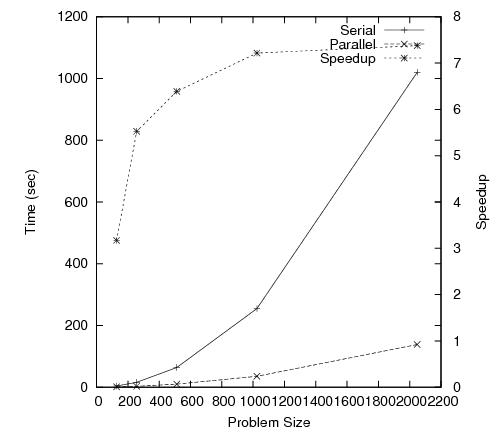
\includegraphics[width=0.7\textwidth]{../data/amazon_n.png}
\caption{Parallel and Serial Timing Results on Amazon EC2 Node with 8 Threads and Static,10 Scheduling and Variable Problem Size}
\label{amazon_n}
\end{figure}

The results from Figure \ref{amazon_threads} showing the effect of varying OpenMP thread count on the 8 core Amazon EC2 node are unsurprising. Each doubling of the number of threads available almost halves the execution time up to 8 threads. Beyond that, no further performance is gained. This is not entirely intuitive: increasing the number of threads beyond the number of cores could increase performance for the Mandelbrot set code if the larger number of threads allowed the sections of the Mandelbrot set to be distributed more evenly. However, these tests were performed with a problem size of 1024 and a chunk size of 10 using static scheduling. From Figure \ref{amazon_threads} timing results we can conclude that the computationally intensive portions of the problem were sufficiently evenly distributed with only 8 threads.

\begin{figure}
\centering
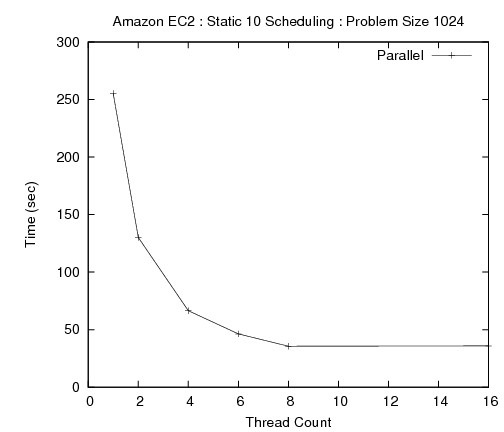
\includegraphics[width=0.7\textwidth]{../data/amazon_threads.png}
\caption{Parallel Timing Results on Amazon EC2 Node with 1024 Problem Size and Static,10 Scheduling and Variable Thread Count}
\label{amazon_threads}
\end{figure}

Finally, Figure \ref{amazon_chunk} shows the effect of varying OpenMP scheduling algorithm and chunk size. While static and dynamic had very similar performance, guided exhibited very strange behavior. Regardless of the chunk size used, guided took approximately the same amount of time. Without knowing the algorithm guided is using to modify the chunk size on the fly, it is difficult to speculate about the cause of this behavior. Presumably, guided was very rapidly settling on the same chunk size in all cases, which would explain the consistent (if poor) results.

\begin{figure}
\centering
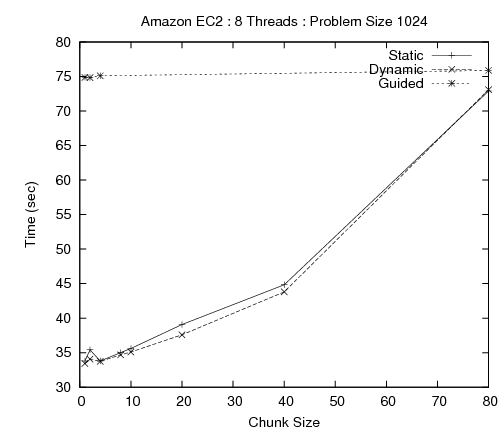
\includegraphics[width=0.7\textwidth]{../data/amazon_chunk.png}
\caption{Parallel Timing Results on Amazon EC2 Node with 1024 Problem Size and 8 Threads and Variable Scheduling}
\label{amazon_chunk}
\end{figure}

Figure \ref{cds_n} provides an interesting contrast to Figure \ref{amazon_n}, both of which demonstrate the effect of increasing problem size. On the Amazon EC2 node, decreasing problem size severely impacted the performance improvement in the parallel code relative to the serial code. On the CDS cluster node, however, the parallel code's performance was slightly less than two times that of the serial code and stayed constant over all problem sizes (the performance improvement varied from 1.994 to 1.907). Because the CDS cluster node has only two cores, it can stay optimally busy much more easily than the 8 core Amazon EC2 node. Of the 8 OpenMP threads used, as long as the two longest running threads have approximately balanced workloads, the CDS node should perform optimally. The Amazon EC2 node, on the other hand, requires hat the eight longest running threads have approximately balanced workloads.

\begin{figure}
\centering
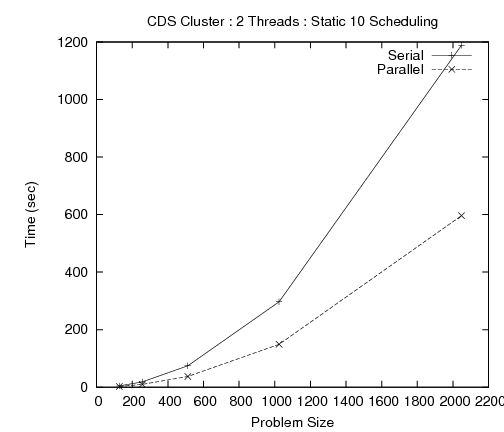
\includegraphics[width=0.7\textwidth]{../data/cds_n.png}
\caption{Parallel and Serial Timing Results on CDS Node with 8 Threads and Static,10 Scheduling and Variable Problem Size}
\label{cds_n}
\end{figure}

There is not much to say about Figure \ref{cds_threads} which shows the effect of modifying the number of OpenMP threads on the CDS node. Because the node has 2 cores, moving from 1 OpenMP thread to 2 roughly doubles performance and further increases yield no additional performance.

\begin{figure}
\centering
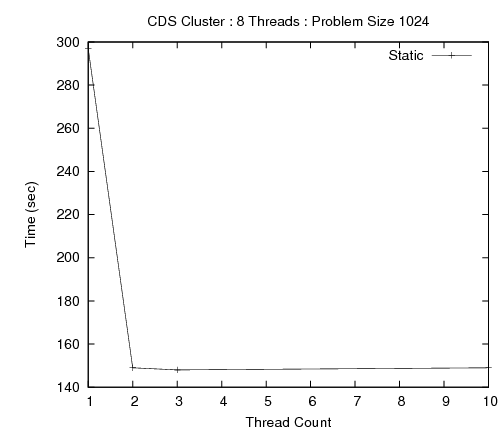
\includegraphics[width=0.7\textwidth]{../data/cds_threads.png}
\caption{Parallel Timing Results on CDS Node with 1024 Problem Size and Static,10 Scheduling and Variable Thread Count}
\label{cds_threads}
\end{figure}

On the other hand, the results of varying the OpenMP scheduling algorithm and chunk size on the CDS cluster node, shown in Figure \ref{cds_chunk}, had very surprising results. Both the static and dynamic scheduling algorithms performed almost identically. However, modifying chunk size yielded very interesting results. I used a much larger range of chunk sizes for the CDS cluster tests than for the Amazon EC2 tests, and found that performance varied quite significantly with chunk size. Predictably, the worst performance was obtained for chunk sizes near the problem size. In these cases, most of the work ended up on a single node, essentially reducing the problem to a serial code. In contrast, the best performance was observed for chunk sizes of less than 100 (with a problem size of 1024). This larger ratio of problem size to chunk size distributed the sections of the Mandelbrot set among the 2 cores more evenly. With chunk sizes in between, however, results were quite varied. With such large chunks, changes in the chunk size could significantly impact which sections of the Mandelbrot set end up on which threads, and certain cases happen to assign large computationally intensive sections to the same thread.

\begin{figure}
\centering
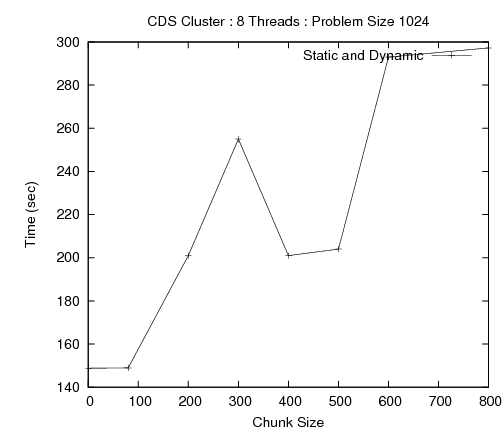
\includegraphics[width=0.7\textwidth]{../data/cds_block.png}
\caption{Parallel Timing Results on Amazon EC2 Node with 1024 Problem Size and 8 Threads and Variable Scheduling}
\label{cds_chunk}
\end{figure}




\section{Output Comparison}

The parallel and serial codes produced identical final Mandelbrot sets.

\end{document}
